\section{Comparaison moteur explosion/réacteur/turbopropusleur en quelques chiffres}

\begin{landscape}
\begin{table}[]
\begin{tabular}{l|l|l|l|}
\cline{2-4}
                                              & \multicolumn{1}{c|}{Moteur a explosion} & Turbopropulseur     & \multicolumn{1}{c|}{Turboréacteur} \\ \hline
\multicolumn{1}{|l|}{Exemple d'aéronef}       & \begin{minipage}{.35\textwidth}
      \begin{figure}[H]
  		\centering
  		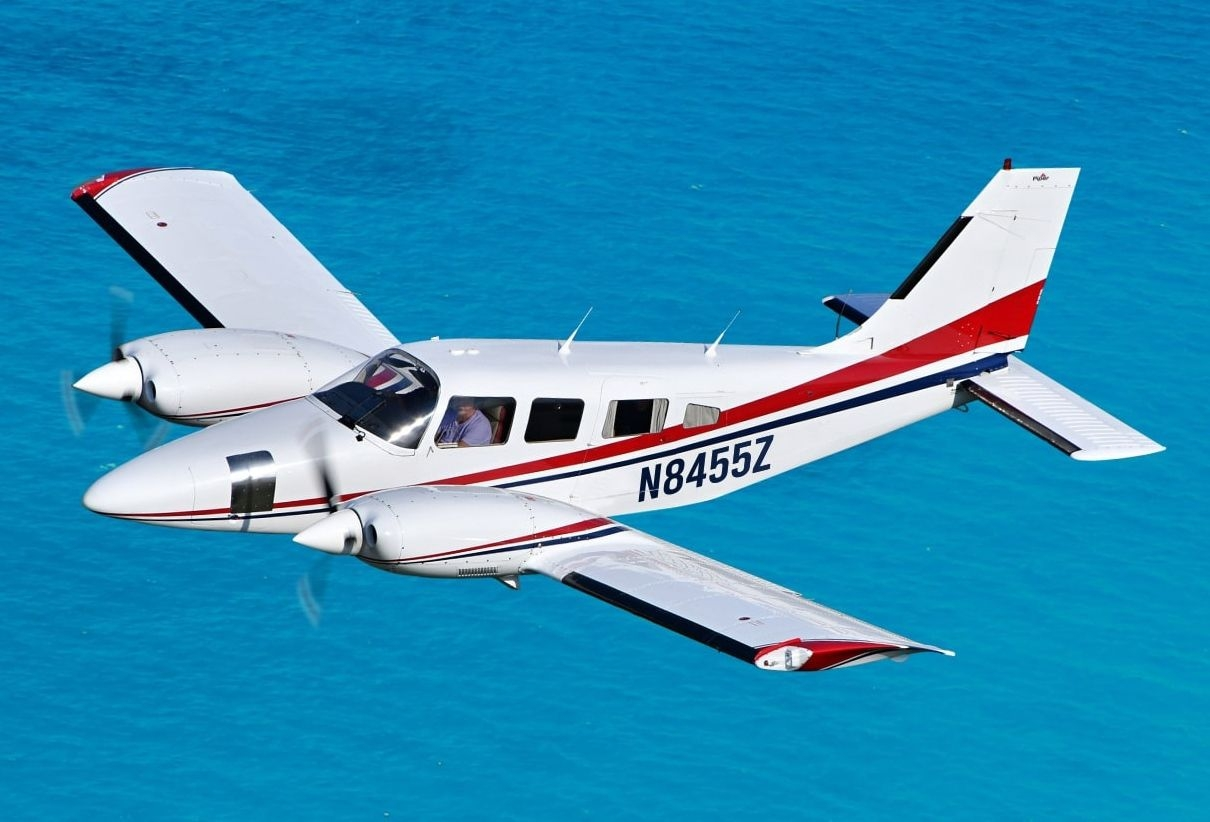
\includegraphics[width=1.0\textwidth]{01-EtudeAeronefs/img/Piper_PA-34.jpg}
  				\legende{Piper PA34}{img:Piper_PA-34}	
		\end{figure}
    \end{minipage}                              
    & \begin{minipage}{.35\textwidth}
      \begin{figure}[H]
  		\centering
  		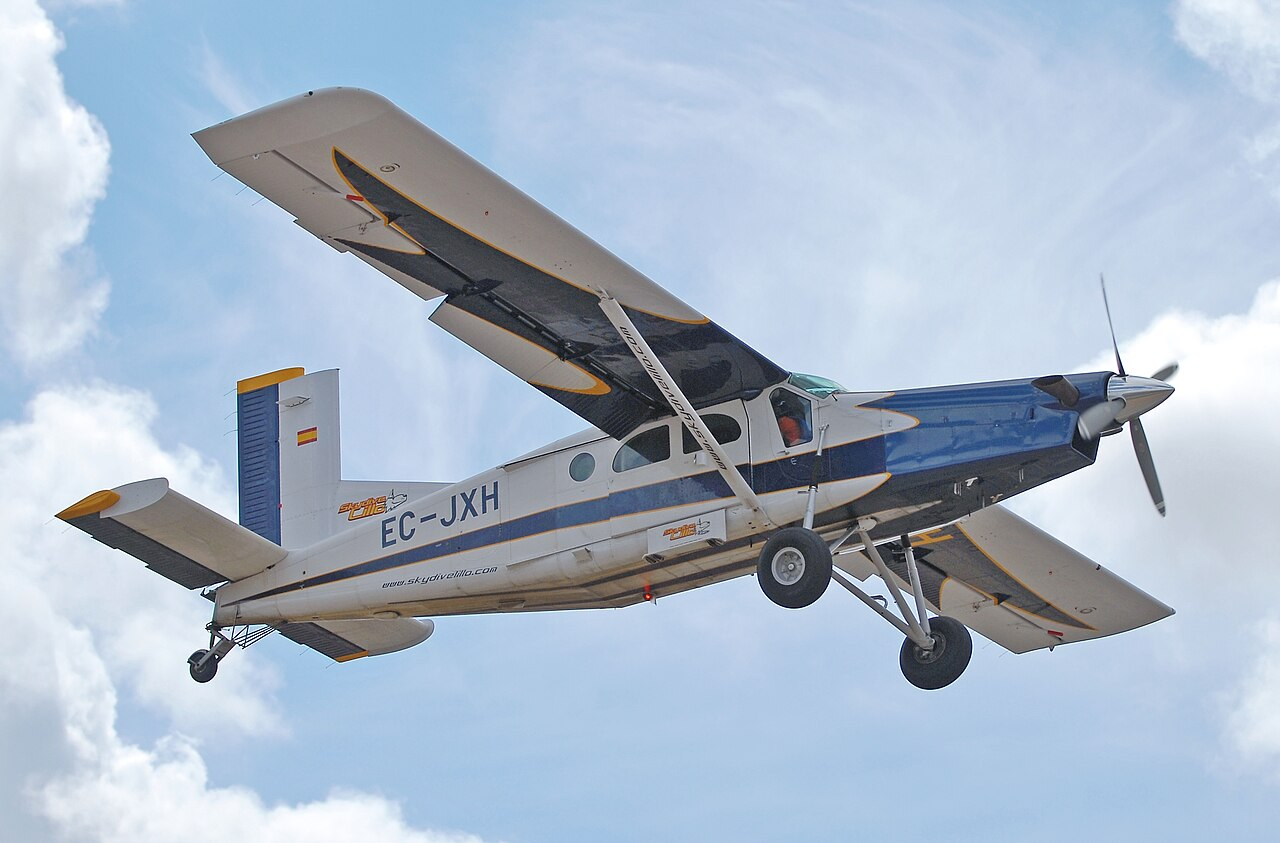
\includegraphics[width=1.0\textwidth]{01-EtudeAeronefs/img/Pilatus_PC-6.jpg}
  				\legende{Pilatus PC6}{img:Pilatus_PC-6}	
		\end{figure}   
		\end{minipage}      
		& \begin{minipage}{.35\textwidth}
      \begin{figure}[H]
  		\centering
  		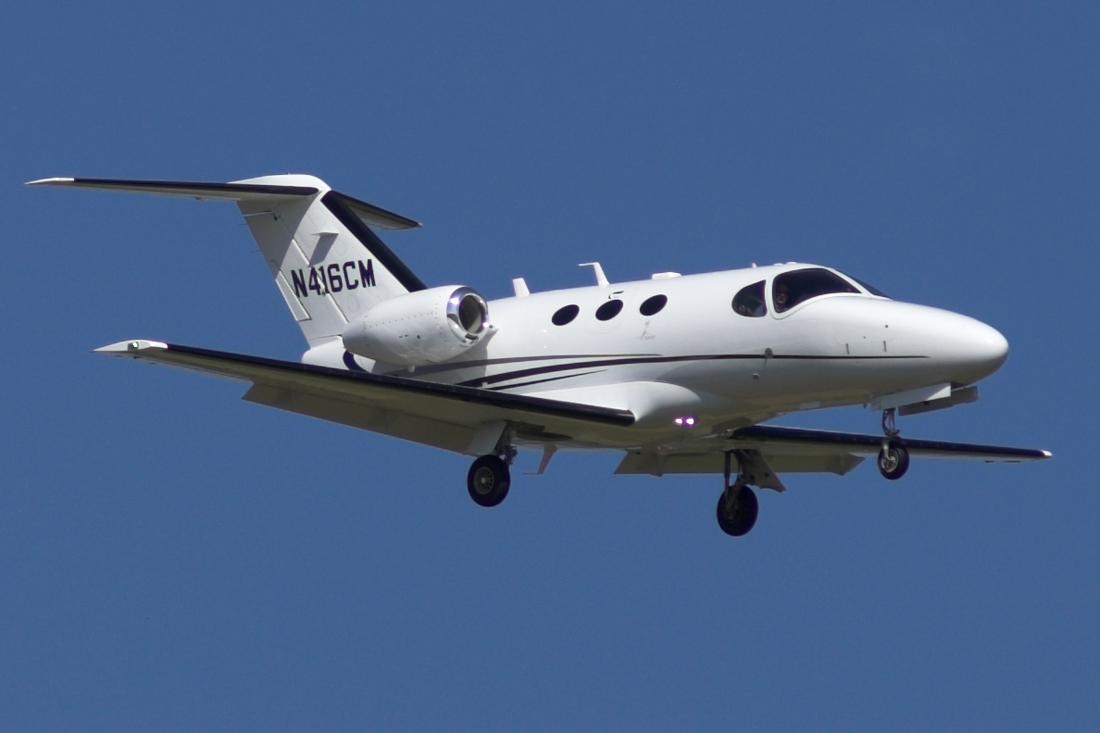
\includegraphics[width=1.0\textwidth]{01-EtudeAeronefs/img/Cessna_Citation_Mustang.jpg}
  				\legende{Cessna Citation Mustang}{img:Cessna_Citation_Mustang}	
		\end{figure}
		\end{minipage}            \\ \hline
\multicolumn{1}{|l|}{Moteur}                  
       & \begin{minipage}{.35\textwidth}
       \begin{figure}[H]
  		\centering
  		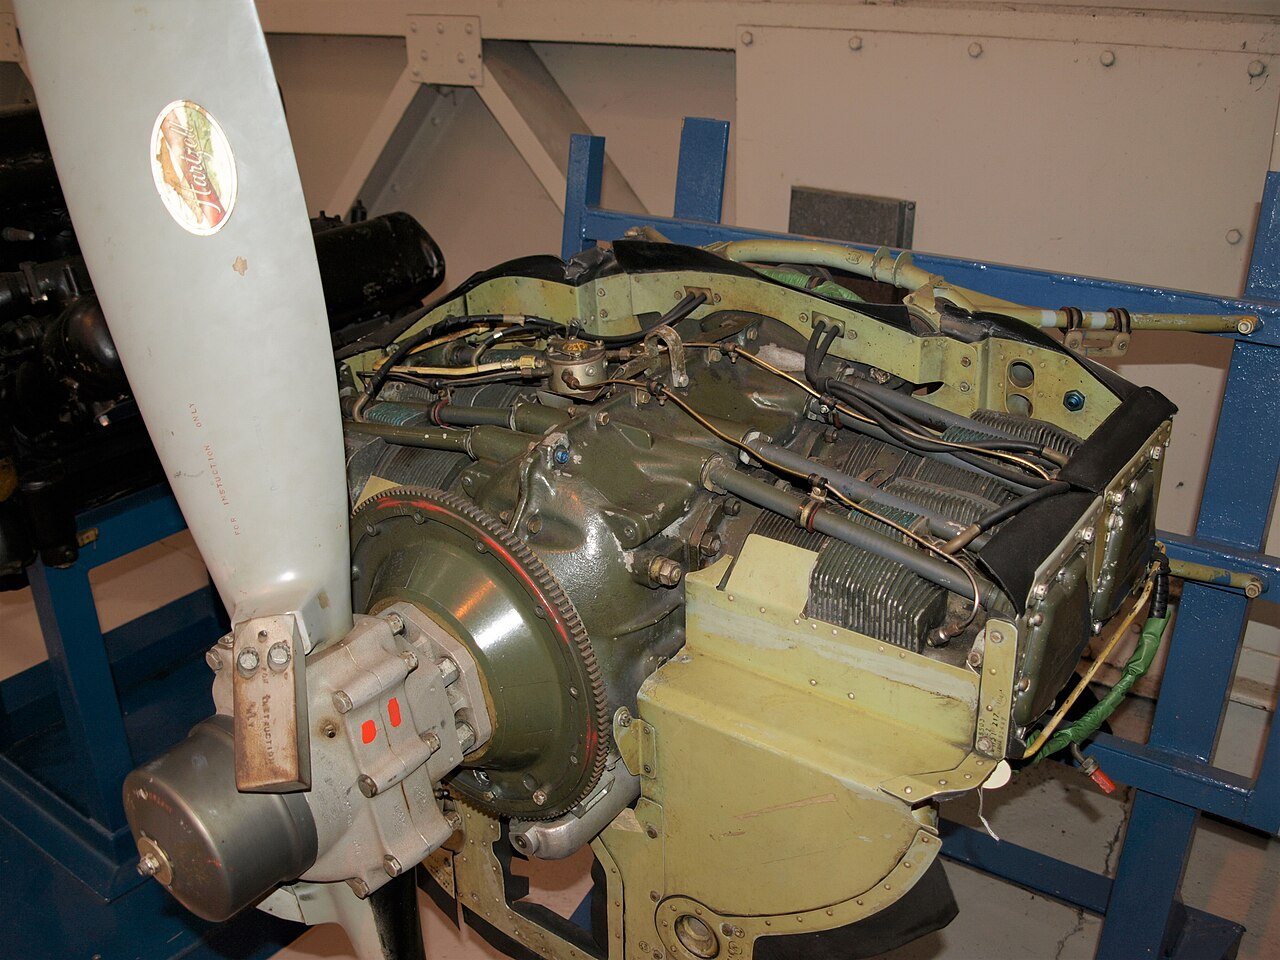
\includegraphics[width=1.0\textwidth]{01-EtudeAeronefs/img/IO360.jpg}
  				\legende{Lycoming IO-360-C1E}{img:IO360}	
		\end{figure}
    \end{minipage}                     
    & \begin{minipage}{.35\textwidth}
    \begin{figure}[H]
  		\centering
  		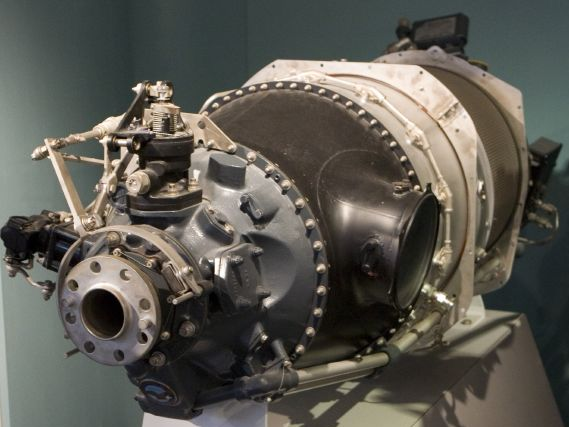
\includegraphics[width=1.0\textwidth]{01-EtudeAeronefs/img/PT6A.jpg}
  				\legende{Pratt\&Whitney PT6A}{img:PT6A}	
		\end{figure}
    \end{minipage} 
    & \begin{minipage}{.35\textwidth}
    \begin{figure}[H]
  		\centering
  		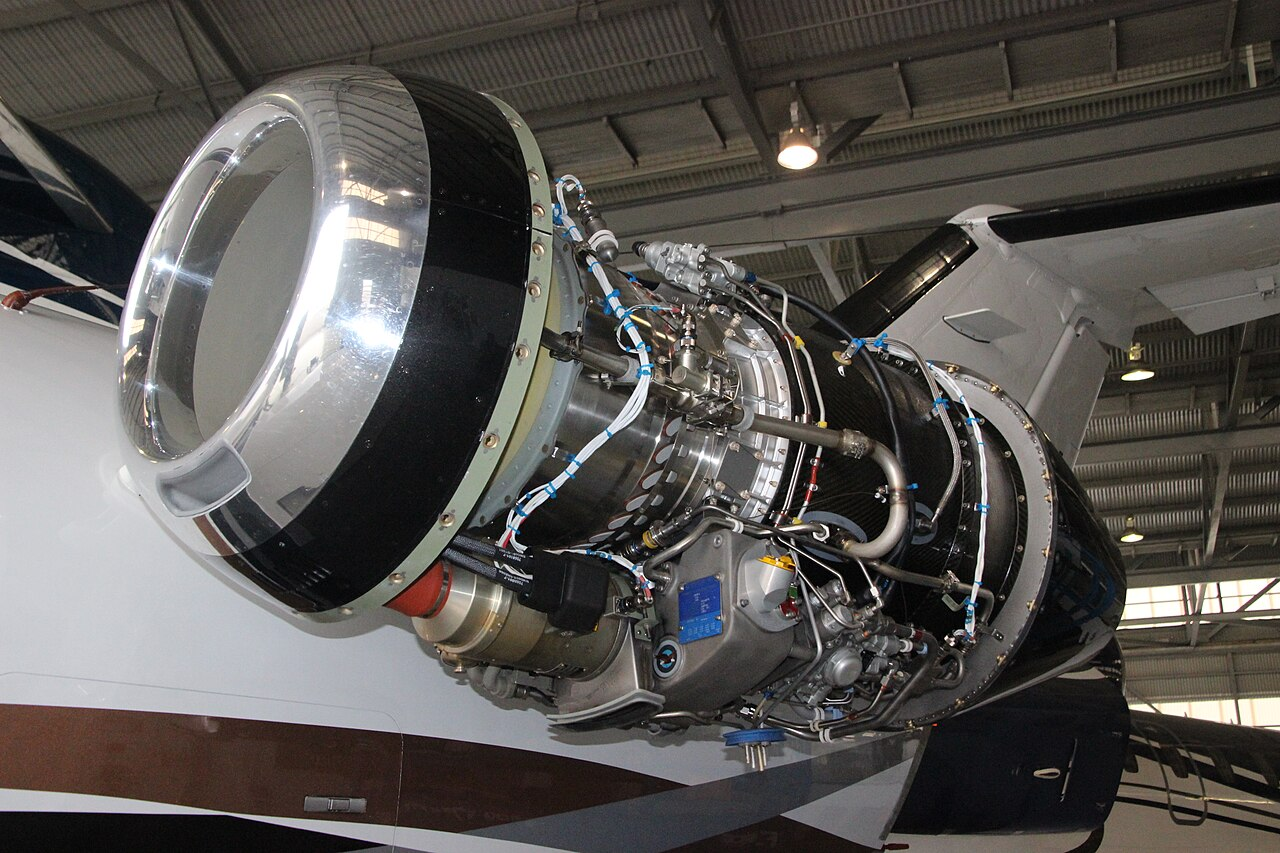
\includegraphics[width=1.0\textwidth]{01-EtudeAeronefs/img/PW615.jpg}
  				\legende{Pratt\&Whitney PW615}{img:PW615}	
		\end{figure}
    \end{minipage}               \\ \hline
\multicolumn{1}{|l|}{Masse}                   & 139 kg                                  & 131 kg              & 140 kg                             \\ \hline
\multicolumn{1}{|l|}{Puissance unitaire}      & 200 CV                                  & 715 CV              & Jusqu'à 1500 CV                    \\ \hline
\multicolumn{1}{|l|}{Rapport masse/puissance} & 1,4 CV/kg                               & 5,5 CV/kg           & 10,7 CV/kg                         \\ \hline
\multicolumn{1}{|l|}{Consommation unitaire}   & 40 L/h                                  & 150 L/h             & 170 L/h                            \\ \hline
\end{tabular}
\caption{Tableau comparant un moteur à explosion, un turboréacteur et un turbopropusleurs de masse similaires (environ 140 kg)}
\end{table}
\end{landscape}